\documentclass{article}

\usepackage[french]{babel}
\usepackage[T1]{fontenc}
\usepackage[letterpaper,top=2cm,bottom=2cm,left=3cm,right=3cm,marginparwidth=1.75cm]{geometry}
\usepackage{amsmath}
\usepackage{graphicx}
\usepackage{enumitem}
\usepackage{subfig}
\usepackage{float}
\usepackage{array}
\usepackage{longtable}
\usepackage{fancyhdr}


\pagestyle{fancy}

\fancyhf{}
\fancyhead[L]{\textbf{INFO—F-202 : Rapport Projet}}
\fancyhead[R]{\textbf{Berthion Antoine, Omelyanyuk Oleksandra}}
\fancyfoot[C]{\thepage}

\usepackage[colorlinks=true, allcolors=blue]{hyperref}

\title{\textbf{INFO—F-202} \\
Langages de Programmation 2 \\ 
Rapport Projet}
\author{Berthion Antoine - 566199 \and Omelyanyuk Oleksandra - 589880}
\date{2 janvier 2025}

\begin{document}

\maketitle

\vspace{-2.5em}

\begin{figure}[H]
    \centering
    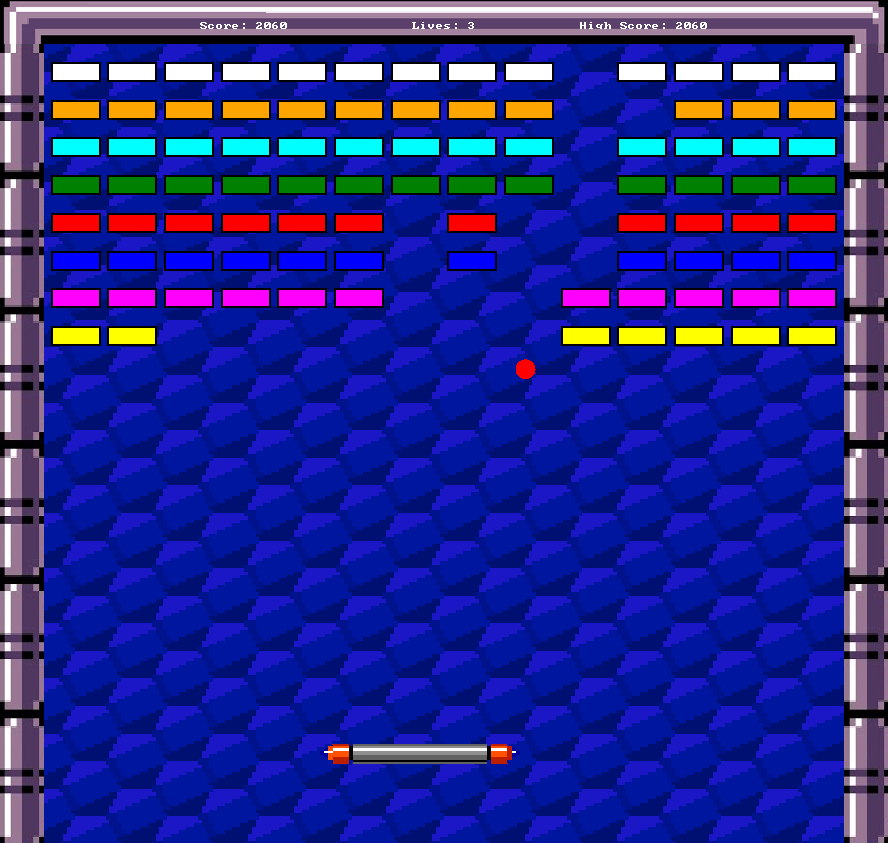
\includegraphics[width=0.5\textwidth]{src/intro.png}
    \label{fig:intro}
    % \caption{Partie classique de notre Arkanoïd}
\end{figure}

\section{Introduction}

\noindent Dans le cadre du cours de \textbf{Langages de Programmation (INFO—F-202)}, nous avons développé un projet prenant pour base le concept du jeu vidéo \textit{Arkanoid}. Ce projet a été implémenté en \textbf{C++} en utilisant la bibliothèque graphique \textbf{Allegro}. 

\noindent L’objectif principal du jeu est de détruire des lignes de briques en les frappant à l’aide d’une balle. Cette balle est contrôlée indirectement par une raquette manipulée par le joueur, ainsi que par les murs environnants qui influent sur sa trajectoire par rebonds. Si la balle quitte l’écran par le bas, une vie est décomptée. Lorsque trois vies sont perdues, la partie se termine par un écran de \textbf{\textit{game-over}} pour le joueur. \\

\noindent De plus, le jeu contient des bonus qui peuvent faciliter l’expérience, ainsi que des niveaux avec une disposition de briques qui varie. \\

\noindent Dans ce rapport, nous détaillerons les tâches exactes implémentées, ainsi que le fonctionnement général du jeu et la structure du code.

\section{Tâches accomplies}

\subsection{Tâches de base}

\noindent Les tâches de base consistaient à concevoir un niveau fonctionnel d’un jeu inspiré d'\textit{Arkanoid}. Pour ce faire, nous avons implémenté les éléments principaux, tels que la raquette, les briques, le score, les vies, et un message de fin de jeu.

\noindent La raquette permet de faire rebondir la balle en modifiant sa trajectoire. La formule utilisée pour déterminer la nouvelle trajectoire est inspirée des consignes initiales, mais a été légèrement ajustée \footnote{En effet, la formule de base ne permettait des angles qu'entre 30° et 120°. Nous l'avons modifiée à des fins de symétrie.} pour rendre les rebonds plus naturels. La direction de la balle après un rebond est donnée par l’angle $\alpha$ calculé selon l’équation suivante : 

\[
\alpha = 30 + 150 \left( 1 - \frac{x}{L} \right),
\]

\noindent où $x$ représente la distance entre le point de contact de la balle et le bord gauche de la raquette, et $L$ correspond à la longueur de la raquette. \\

\noindent Les briques sont affichées à l’écran en fonction des données lues depuis un fichier au format \textit{.map}. Ce format de fichier spécifie leur position relative et pourra être amélioré ultérieurement pour inclure le type de chaque brique et les informations relatives aux bonus. Cette structure facilitera la création de différents niveaux et permettra une personnalisation aisée de la disposition des briques.

\noindent Le score et le nombre de vies restantes sont affichés en haut de l’écran pendant toute la durée de la partie. Lorsque la partie se termine, un message indiquant le score final s’affiche, offrant également la possibilité de redémarrer le jeu en appuyant sur la touche \textit{Entrée}.


\subsection{Tâches additionnelles}
\label{subsec:additionaltasks}

\noindent Après avoir implémenté la base du jeu, nous avons ajouté plusieurs fonctionnalités supplémentaires. \\

\noindent Premièrement, nous avons défini différents types de briques et intégré cette information dans les fichiers déterminant leur disposition. Cela inclut notamment :  
\begin{itemize}
    \item les \textbf{briques argentées}, qui nécessitent deux coups pour être détruites ;
    \item les \textbf{briques dorées}, qui sont indestructibles.
\end{itemize}
\noindent Chaque type de brique est associé à un score spécifique. Cette structure a également permis d’intégrer un système de meilleur score, sauvegardé dans le fichier \textit{highscore.txt}. Ce meilleur score est conservé entre les sessions du jeu, affiché en haut de l’écran aux côtés des vies et du score actuel, et peut être réinitialisé en appuyant sur la touche \textbf{R}. \\

\noindent Grâce à ces options, il est possible de concevoir des niveaux variés comportant des briques de différents types. Dans le jeu, les niveaux se succèdent automatiquement lorsqu’un niveau est complété (toutes les briques destructibles ont été éliminées). Il est également possible de changer manuellement de niveau en appuyant sur les flèches gauche ou droite du clavier. \\

\noindent Par ailleurs, nous avons ajouté une fonctionnalité permettant de contrôler la raquette avec la souris, en plus des touches du clavier. Ces deux modes de contrôle sont disponibles simultanément. Le jeu vérifie d'abord l’état du clavier et, si aucune touche n’est activée, il prend en compte les mouvements de la souris vers la gauche ou la droite. \\

\noindent Finalement, des \textbf{bonus} ont été ajoutés au jeu. Ces bonus peuvent être contenus dans des briques, et l’information correspondante est également stockée dans les fichiers \textit{.map}. Lorsqu’un bonus est présent, une lettre l’indique sur la brique associée. Les bonus implémentés sont les suivants : 
\begin{itemize}
    \item \textbf{Laser} : des lasers peuvent être tirés depuis la raquette vers le haut de l’écran, détruisant toutes les briques touchées, sauf les dorées. 
    \item \textbf{Agrandir} : la raquette devient plus large.
    \item \textbf{Attraper} : la raquette attrape la balle, qui peut être relâchée en appuyant sur la touche \textbf{Espace}. Si aucune action n’est effectuée, la balle se relâche automatiquement après un certain temps.
    \item \textbf{Ralentissement} : la balle se déplace plus lentement pendant un temps limité.
    \item \textbf{Interruption} : la balle se divise en trois. Aucune vie n’est perdue si deux des trois balles tombent.
    \item \textbf{Joueur} : une vie supplémentaire est accordée au joueur.
\end{itemize}

\noindent Aucun bonus n’a d’effet cumulatif, à l’exception du bonus de ralentissement. Lorsqu’un nouveau bonus est attrapé, l’effet du précédent est annulé.



\section{Classes et logique du jeu}

\noindent Dans cette partie du rapport, nous développerons davantage l'implémentation du jeu ainsi que la logique générale. 

\noindent Nous nous baserons sur le diagramme des classes ci-dessous dans la figure \ref{fig:cdgm} pour présenter la structure générale du jeu et expliquer les classes implémentées plus en profondeur, ainsi que leurs interactions.

\vspace{1em}

\begin{figure}[H]
    \hspace{-1.5cm} % tweaking, kinda
    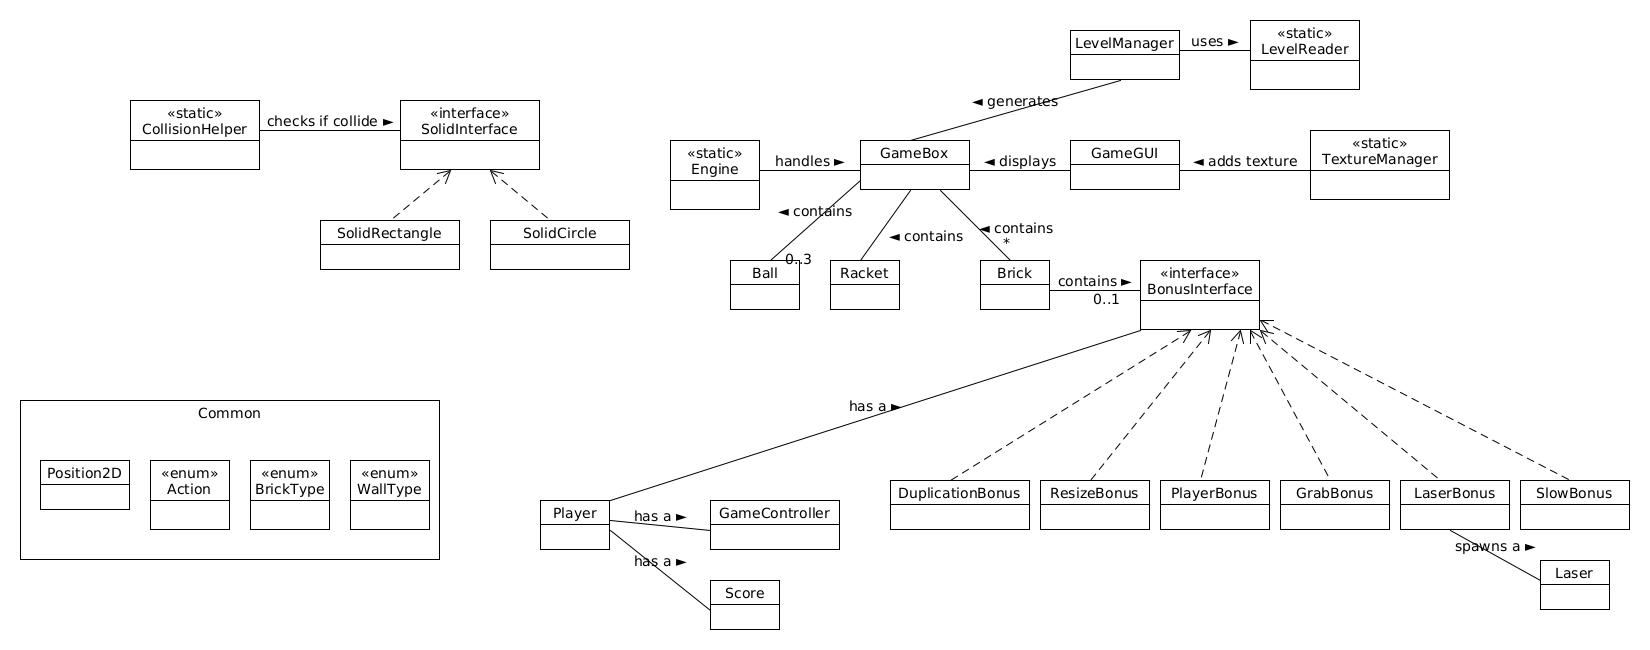
\includegraphics[width=1.2\textwidth]{src/class_diagram.jpg}
    \caption{Diagramme de classe du projet Arkanoïd}
    \label{fig:cdgm}
\end{figure}

\noindent Nous allons décrire brièvement les différentes classes ainsi que leur fonctionnement.

\subsection{SolidInterface}
\label{subsec:solidinterface}

\noindent La classe \textbf{SolidInterface} est une interface qui regroupe les objets possédant des \textbf{\textit{hitboxes}}, c'est-à-dire des zones de collision. Bien que la classe ne gère pas directement ces interactions, elle facilite la détection des collisions entre objets solides. Cette interface est implémentée par la classe \textbf{SolidRectangle}, utilisée par les briques, la raquette et les bonus (décrits dans les sous-sections suivantes), ainsi que par \textbf{SolidCircle}, utilisée pour l'objet \textbf{Ball}. Les classes qui réalisent cette interface doivent implémenter les méthodes abstraites afin de compléter l'interface et être utilisées par le reste du code.

\subsection{CollisionHelper}

\noindent La classe statique \textbf{CollisionHelper} vient en aide à \textbf{SolidInterface} en facilitant la détection des collisions entre les objets qui implémentent cette interface. Ainsi, \textbf{CollisionHelper} est capable de gérer les collisions entre toutes les paires d'objets réalisant l'interface \textbf{SolidInterface}. Cette approche modulaire permet d'ajouter rapidement le support pour de nouveaux types d'objets solides, en les faisant simplement hériter de l'interface \textbf{SolidInterface}, tout en ajoutant les méthodes de détection de collisions avec les autres objets dans \textbf{CollisionHelper}.

\subsection{Objets du jeu (Ball, Racket et Brick)}

\noindent Les classes \textbf{Ball}, \textbf{Racket} et \textbf{Brick} représentent respectivement les objets de même nom dans le jeu. Chacun de ces objets dispose d'une hitbox, implémentée via l'interface \textbf{SolidInterface}, que nous avons abordée dans la sous-section \ref{subsec:solidinterface}. Ces objets possèdent également des attributs permettant de gérer leur vitesse, ainsi qu'une \textbf{Position2D} pour assurer leur déplacement dans l'espace de jeu.

\subsection{Objets liés au Joueur (Player, GameController, Score)}

\noindent Les classes \textbf{Player}, \textbf{GameController} et \textbf{Score} gèrent les informations relatives au joueur. La classe \textbf{GameController} permet à l'\textbf{Engine} du jeu de récupérer la configuration des touches et, grâce à elle, d'interpréter les appuis de touches de l'utilisateur pour les transformer en actions. Quant à la classe \textbf{Player}, elle agit comme un conteneur pour les données liées à l'utilisateur, telles que le score actuel. Elle stocke également le nombre de vies du joueur, l'objet actuellement dans son inventaire, l'état de sa raquette, ainsi que d'autres valeurs nécessaires au bon déroulement de la partie. L'accès au score et au \textbf{GameController} se fait via l'objet \textbf{Player}, facilitant ainsi l'accès à ces informations en passant en paramètre uniquement un pointeur vers l'objet \textbf{Player}.

\subsection{LevelManager et LevelReader}

\noindent Ces classes simples sont essentielles pour la lecture et la gestion des niveaux du jeu. La classe \textbf{LevelReader} permet de lire les fichiers au format \texttt{.map} selon l'encodage décrit dans la section \ref{subsec:additionaltasks}. Elle crée ainsi des objets \textbf{GameBox}, dont les détails sont présentés dans la section \ref{subsec:gamebox}. La classe \textbf{LevelManager} gère l'avancée de l'utilisateur à travers les niveaux. Elle permet de changer facilement la \textbf{GameBox} actuelle en modifiant le pointeur correspondant, en passant en paramètre une référence vers celui-ci. Cette opération de changement de niveau est effectuée par le \textbf{GameEngine}. Les chemins vers les fichiers des niveaux sont stockés dans un vecteur, à travers lequel l'utilisateur va boucler. Lorsque le dernier niveau est terminé, le jeu revient automatiquement au premier niveau.

\subsection{Interface visuelle (GameGUI et TextureManager)}

\noindent L'interface visuelle constitue une part importante de notre projet. Toutefois, elle est séparée de la logique du jeu et n'a aucune connaissance de ce qui se passe en son sein. En effet, elle ne connaît pas les règles du jeu et reçoit uniquement des instructions concernant les éléments à afficher, à partir des informations sur l'état de la partie. L'interface visuelle utilise un \textbf{TextureManager} pour récupérer efficacement les textures du jeu et les afficher. Ces textures sont chargées à partir d'images bitmap via la bibliothèque graphique \textbf{Allegro}. Une fois chargées, elles ne sont plus rechargées, ce qui permet de réduire l'usage des ressources et d'optimiser les performances.

\subsection{GameBox}
\label{subsec:gamebox}

\noindent La \textbf{GameBox} est le conteneur principal de notre projet. Elle a en effet accès à la raquette, aux balles, ainsi qu'aux briques, qu'elles soient équipées ou non de bonus. La GameBox conserve également des informations sur les éventuels lasers ou bonus présents à l'écran. En plus de ces objets, la GameBox dispose de plusieurs méthodes permettant d'interagir avec eux. Toutefois, elle ne possède aucune connaissance sur le fonctionnement global du jeu. En effet, elle est limitée à des méthodes d'interaction avec les objets mentionnés précédemment. Toute la logique du jeu est centralisée et gérée par le cœur du jeu, le \textbf{GameEngine}, décrit dans la sous-section suivante.

\subsection{GameEngine}

\noindent Le \textbf{GameEngine} constitue le moteur de notre jeu. Il est le seul à connaître les règles du jeu. Ainsi, à chaque frame, la méthode dédiée au "tour de logique" est appelée. L'engine se charge de plusieurs tâches essentielles : il vérifie les collisions, applique les réactions appropriées (comme retirer des vies aux briques, faire rebondir la balle, déplacer un laser, etc.), et gère les entrées du joueur via le \textbf{GameController}. Il évalue également l'état de la partie (victoire ou défaite), applique la logique des bonus actifs, et met à jour les variables du joueur, telles que le score et le nombre de vies. \\

\noindent La centralisation de la logique dans le \textbf{GameEngine} permet de faciliter l'ajout de nouveaux objets interagissant avec les autres, sans avoir à modifier les autres classes. En effet, toutes les interactions se font via le moteur de jeu, ce qui simplifie grandement l'implémentation et la maintenance du code.

\subsection{BonusInterface}

\noindent Dans cette sous-section, nous aborderons brièvement la gestion des bonus. À l'instar de l'interface \textit{SolidInterface}, nous avons souhaité regrouper les différents types de bonus sous une interface commune. Toutefois, le contrat de l'interface \textbf{BonusInterface} est moins contraignant : il garantit simplement que les bonus pourront appliquer et annuler leur logique à l'aide de deux méthodes, \texttt{applyLogic} et \texttt{revertLogic}. Cette approche simplifie grandement l'implémentation des différents types de bonus. 

\noindent En plus de ces méthodes, \textbf{BonusInterface} contient certains attributs utiles à la gestion de la logique des bonus, tels que le flag \texttt{isActive} ou le \texttt{TTL} (Time To Live), qui détermine la durée de vie du bonus. Bien que ces attributs soient utiles, leur utilisation n'a pas toujours été optimale, faute de temps. \\

\noindent Nous évoquerons aussi le cas particulier du \textbf{Bonus Laser}, qui permet l'apparition de lasers à l'écran. Ce bonus nécessite un traitement spécifique dans le \textbf{GameEngine} pour générer et gérer les lasers. Cependant, il aurait été possible de gérer cette logique directement dans le bonus, mais par manque de temps, nous avons préféré centraliser cette logique dans le \textbf{GameEngine}. Cette incohérence résulte d'un choix structurel qui aurait pu être optimisé si le projet en avait permis une gestion plus souple des bonus.






\section{Modèle-Vue-Contrôleur}

\noindent Dans cette section, nous discuterons de l'application du modèle \textbf{Modèle-Vue-Contrôleur} (MVC) dans notre implémentation du projet.

\noindent L'architecture Modèle-Vue-Contrôleur se compose de trois parties distinctes : la vue, le contrôleur et le modèle. Nous allons expliquer comment chaque composant est représenté dans notre projet.

\subsection{Modèle}

\noindent Le \textbf{modèle} contient les données principales du jeu, telles que les objets du jeu (balles, briques, raquette, etc.), les scores, et les vies restantes (par l'intermédiaire de l'objet \textbf{Player}). Dans notre projet, le modèle est représenté par la classe \texttt{GameBox}. Cette classe agit comme un conteneur pour ces données et inclut des méthodes pratiques permettant de manipuler et de modifier ces informations. La logique du jeu (telles que les règles concernant les collisions et les bonus) ainsi que l'affichage (via la vue) sont séparés de la \texttt{GameBox}, ce qui permet à celle-ci de se concentrer uniquement sur la gestion des données, tout en étant utilisée par le contrôleur et la vue.

\subsection{Vue}

\noindent La \textbf{vue} dans notre architecture correspond à la présentation graphique de l'application. Elle est responsable de l'affichage des informations à l'utilisateur, sans connaissance des règles du jeu ou de la logique interne. Dans notre projet, cette fonction est assurée par la classe \texttt{GameGUI}, munie de son \texttt{TextureManager}. La vue ne gère que l'affichage des données fournies par le modèle et reste totalement découplée de la logique du jeu.

\subsection{Contrôleur}

\noindent Le \textbf{contrôleur} est chargé de la gestion de la logique du jeu et des actions de l'utilisateur. Dans notre architecture, la classe \texttt{GameEngine} joue le rôle principal du contrôleur. Elle est responsable de la mise à jour de l'état du jeu en fonction des actions de l'utilisateur (comme les entrées clavier ou souris) et de la logique de jeu (gestion des collisions, calcul des scores, etc.). En d'autres termes, \texttt{GameEngine} modifie l'état du modèle, coordonne l'interaction entre la vue et le modèle et assure le bon déroulement du jeu.

\section{Utilisation des LLM}

\noindent Dans cette courte partie, nous discuterons de l'utilisation des LLM dans le cadre du projet. Aucun LLM n'a été utilisé pour l'aspect implémentation ainsi que la compréhension du projet. Cependant, ce rapport à été corrigé du point de vue de la syntaxe et de la grammaire par DeepL ainsi qu'un modèle GPT. Notons tout de même qu'aucune des informations du rapport n'a été produite par une autre personne que l'auteur.

\section{Conclusion}

\noindent Ce projet a permis de mettre en œuvre une version du jeu \textit{Arkanoid} en utilisant le langage C++ et la bibliothèque graphique Allegro. À travers l'implémentation de diverses fonctionnalités telles que la gestion des collisions, des bonus, et des niveaux, nous avons pu développer un jeu complet et fonctionnel. \\

\noindent L'architecture Modèle-Vue-Contrôleur a joué un rôle crucial dans la séparation des responsabilités, facilitant ainsi l'extension du jeu et la maintenance du code. En intégrant différentes mécaniques de jeu et en offrant une interface graphique intuitive, nous avons abouti à un projet à la fois technique et ludique. Ce travail met en lumière l'importance de la modularité dans la conception de jeux vidéo et permet de mieux comprendre les interactions entre les différents composants d'une application complexe.

\end{document}
